%!TEX encoding = UTF-8 Unicode
\documentclass[12pt]{article} 
\usepackage[left=0.75in,top=0.7in,right=0.75in,bottom=0.3in]{geometry} % Document margins
\usepackage{CJK}
\usepackage{graphicx}
\usepackage{mathtools}
\usepackage{mathrsfs}
\usepackage{amssymb}
\usepackage{hyperref}

\makeatletter
\renewenvironment{itemize}
{\list{$\bullet$}{\leftmargin\z@ \labelwidth\z@ \itemindent-\leftmargin
\let\makelabel\descriptionlabel}}
{\endlist}
\makeatother

\begin{CJK}{UTF8}{bsmi}
\title{\textbf{Homework1 / Linear Binary Perceptron}}
\author{\textbf{李豪韋 (HW-Lee) ID 103061527}}
\date{}

\begin{document}
\vspace*{-60pt}
    {\let\newpage\relax\maketitle}

\section*{Overview}
\vspace{-20pt}
\noindent\makebox[\linewidth]{\rule{\textwidth}{0.4pt}}
\vspace{5pt}

The homework consists of two parts: 1) Implement a perceptron which is able to tell data with positive labels from those with negative labels; and 2) Calculate the weights, which can be simply regarded as correlation, between students features (namely gender, activities, tests, and participation) in a course and final consequences (pass or fail) of them. \\

In the first part, a matlab script $\mathsf{Hw1\_LinBinPerc\_DataGen.m}$ is needed to generate a random set of data with binary labels so that the data are known to be linearly separable. Then, the task is to pretend that the linear weight are unknown and train the perceptron with some algorithm iteratively. \\

In the second part, there is a given excel file $\mathsf{NN\_RealDataForHW1.csv}$ that contains grade information from a real NTHU course (obfuscated to hide the identity of students). Each column contains the grades for an activity, and the task is to discover how these columns were linearly combined to determine whether a student has passed (P) or failed (F). The code developed for the first part can be used in this part, and the final weights and bias in the trained perceptron should be shown in the report. \\

Note: For the second part, the following MATLAB functions may be useful: $\mathsf{csvread()}$, $\mathsf{importdata()}$. \\

\section*{Implementation}
\vspace{-20pt}
\noindent\makebox[\linewidth]{\rule{\textwidth}{0.4pt}}

\begin{enumerate}
	\item {\bf Functions}
	\begin{itemize}
		\item {\bf Hw1PerceptronClassifier.train(X, y)} \\ \\
			Return a reference of a perceptron classifier trained with training set $X$ and corresponded ground truths $y$. \\
		\item {\bf Hw1PerceptronClassifier.predict(X)} \\ \\
			Return a binary vector contains elements with value of either -1 or 1, which refers to predicted results with unknown testing set $X$. \\
		\item {\bf Hw1PerceptronClassifier.visualInfo()} \\ \\
			Show the property of a classifier in a visual way, including parameters $w$, $b$, and all $w's$ and $b's$ during training process.
	\end{itemize}
	\newpage
	\item {\bf Process}
	\begin{itemize}
		\item {\bf Generate training set $X$ and corresponded ground truths $y$} \\ \\
			Combine two matrices $\mathsf{class0}$ and $\mathsf{class1}$ into a matrix vertically, and generate a vector which contains the 
			'class label' indicating which class each row instance belongs to. (-1 refers to $\mathsf{class0}$ and 1 to $\mathsf{class1}$) \\
		\item {\bf Initialize parameters of the perceptron classifier} \\ \\
			In default, the parameters, namely $w$ and $b$, will be zero vector and zero respectively. \\
		\item {\bf Iterate algorithm with N times}
		\begin{align*}
			&\text{Predict labels with current parameters}: \, z=Xw+b \\
			&\text{Find the set consisting of all} \\
			&\quad \text{incorrectly predicted instances}: \, errIdx = \{i|z_i \neq y_i \,\, \forall i=1, \cdots, N \} \\
			&\text{Update parameters}: \, 
			\begin{pmatrix}w_{\text{new}} \\ b_{\text{new}}\end{pmatrix} = 
			\begin{pmatrix}w \\ b\end{pmatrix} + \sum_{i \in errIdx}y_i
			\begin{pmatrix}x^{(i)} \\ 1\end{pmatrix}
		\end{align*}
	\end{itemize}
\end{enumerate}

\section*{Results}
\vspace{-20pt}
\noindent\makebox[\linewidth]{\rule{\textwidth}{0.4pt}}

\hspace*{-14em}
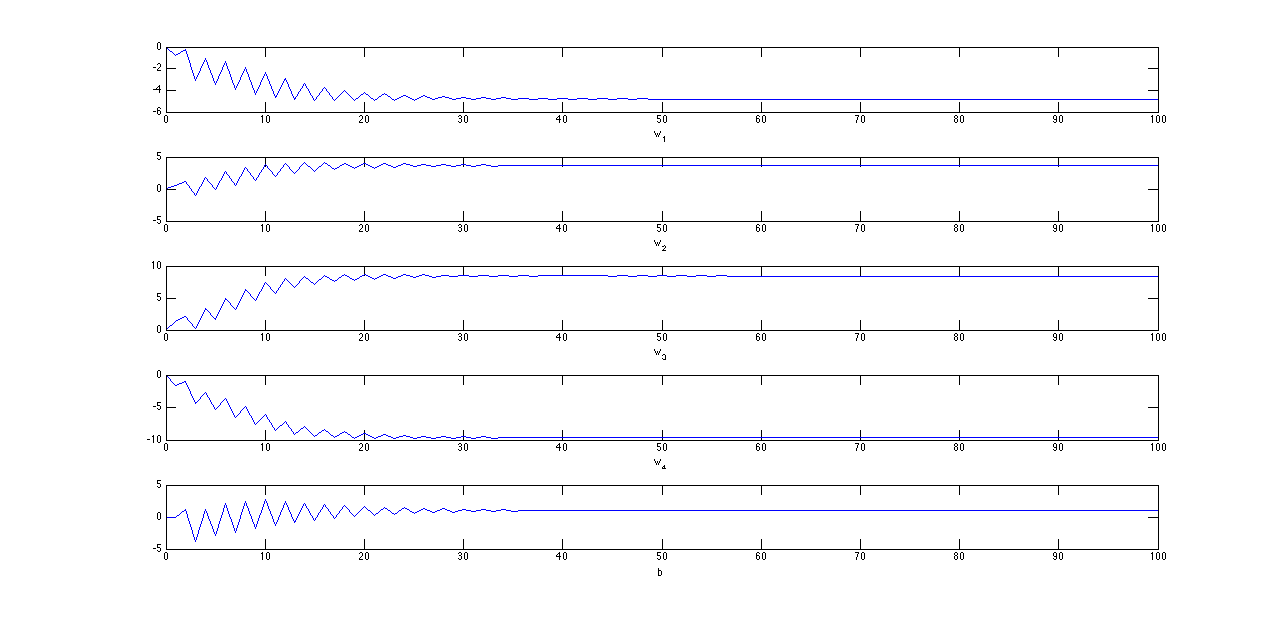
\includegraphics[scale=.6]{../res/part1_parametrogram_init0.png}
\vspace*{-4.5em}
\begin{center}
[Fig.1: Parametrogram in part I]
\end{center}

\vspace*{-4.5em}
\begin{center}
[Fig.2: Evaluated values distribution in part I]
\end{center}
\vspace*{-1em}
\hspace*{-12em}
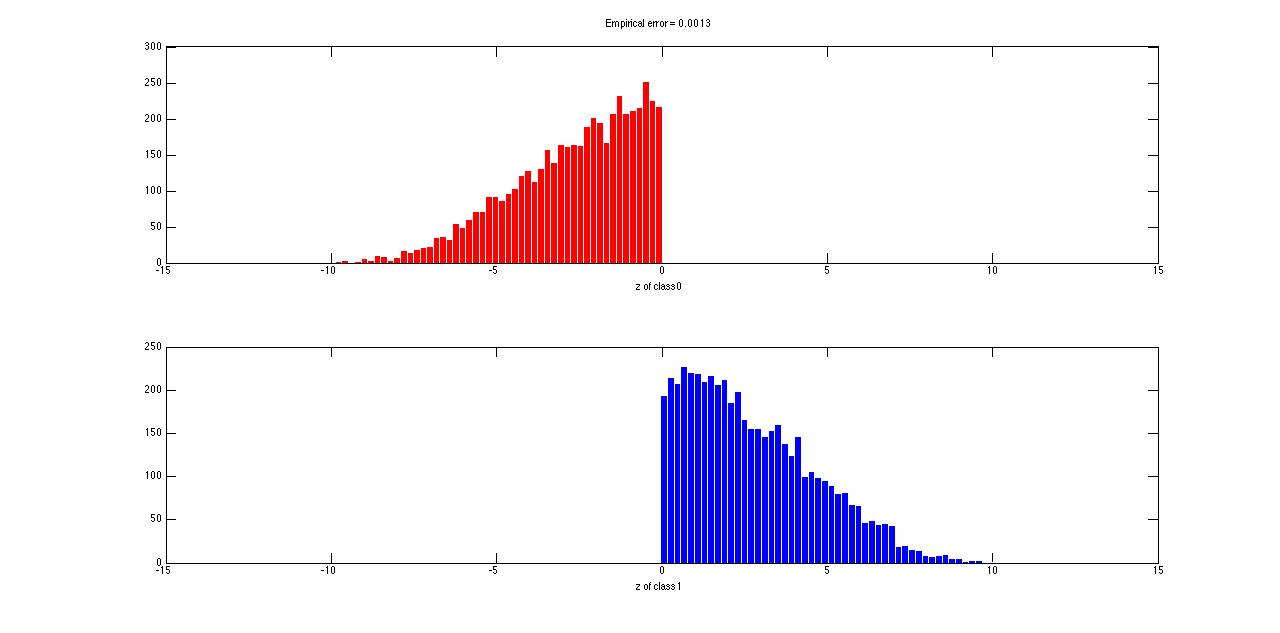
\includegraphics[scale=.59]{../res/part1_distributionDiag.png}

\vspace*{-2em}
\hspace*{-12.5em}
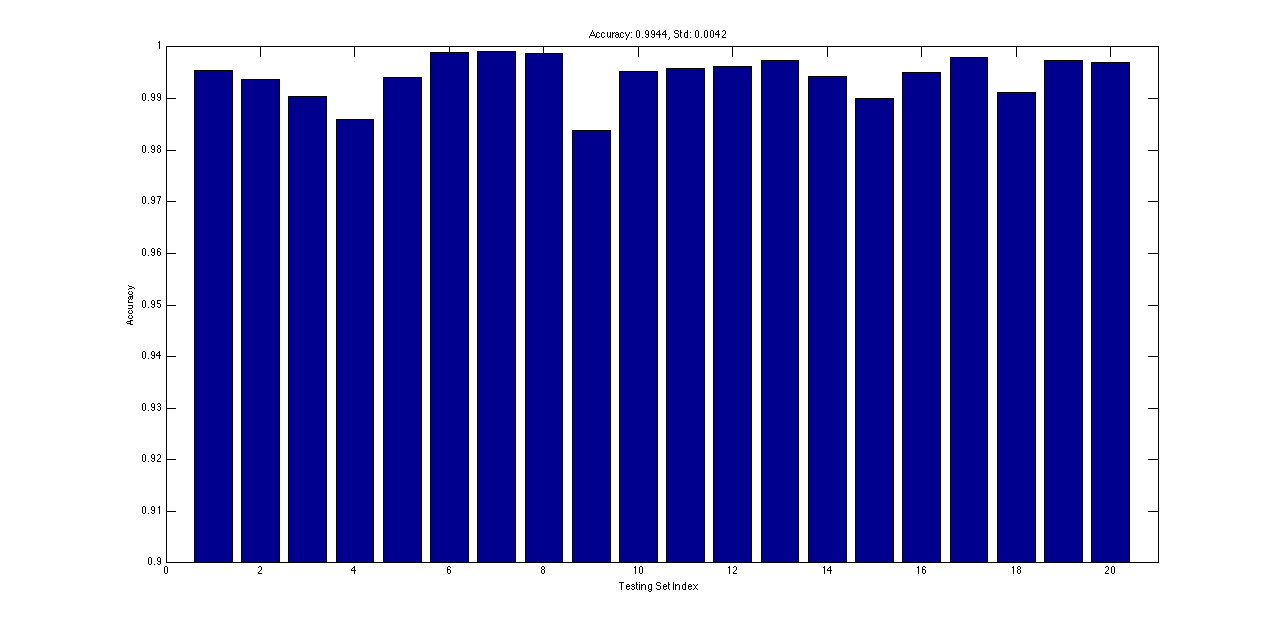
\includegraphics[scale=.58]{../res/part1_performance.png}
\vspace*{-4em}
\begin{center}
[Fig.3: Accuracy of 20 different data sets generated by $\mathsf{Hw1\_LinBinPerc\_DataGen.m}$]
\end{center}
\newpage
\vspace*{-1.5em}

In the first part, there are 3 visual results: 1) "parametrogram", a iteration-value figure which shows the value of parameters at each iteration; 2) values computed by the classifier of both $\mathsf{class0}$ and $\mathsf{class1}$; 3) accuracy with 20 different data sets to evaluate performance. After simulation, there are several conclusions can be figured out:
\begin{itemize}
	\item parameters can get converged with a large iteration time and a proper learning rate $\eta$.
	\item generally, empirical error is difficult to be zero.
	\item performance is roughly $99.45 \pm 0.38 \%$.
\end{itemize}

\vspace*{-0.8em}
\hspace*{-13em}
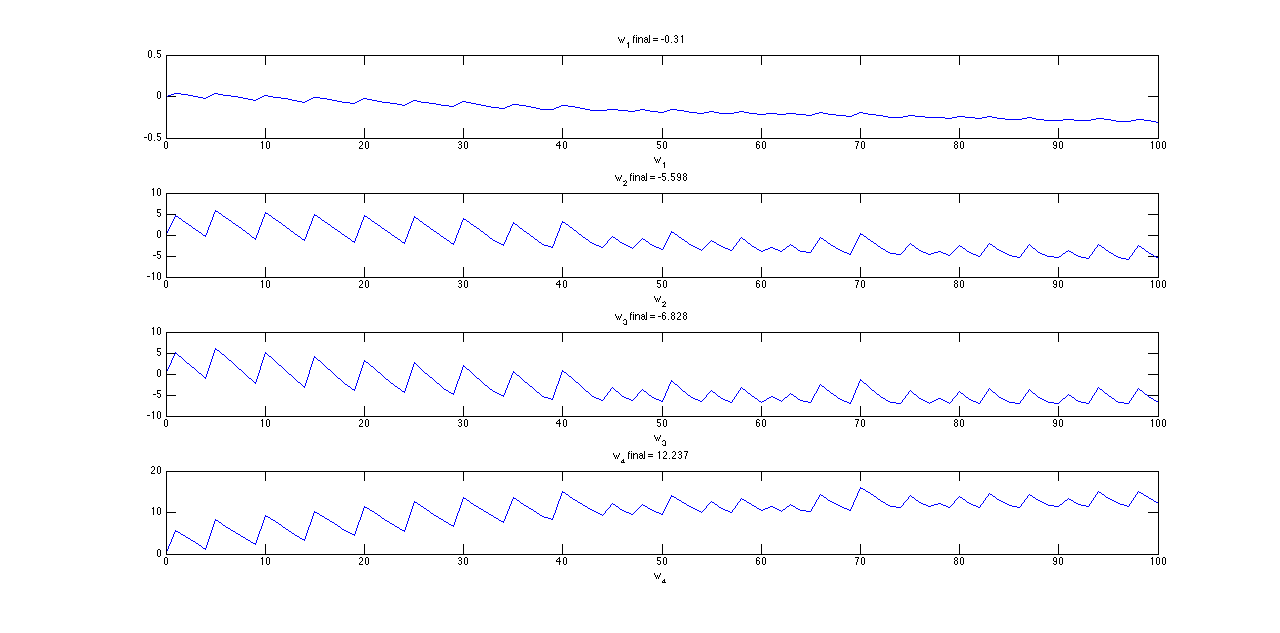
\includegraphics[width=26.5cm,height=8cm]{../res/part2_parametrogram1_init0.png}

\vspace*{-2em}
\hspace*{-13em}
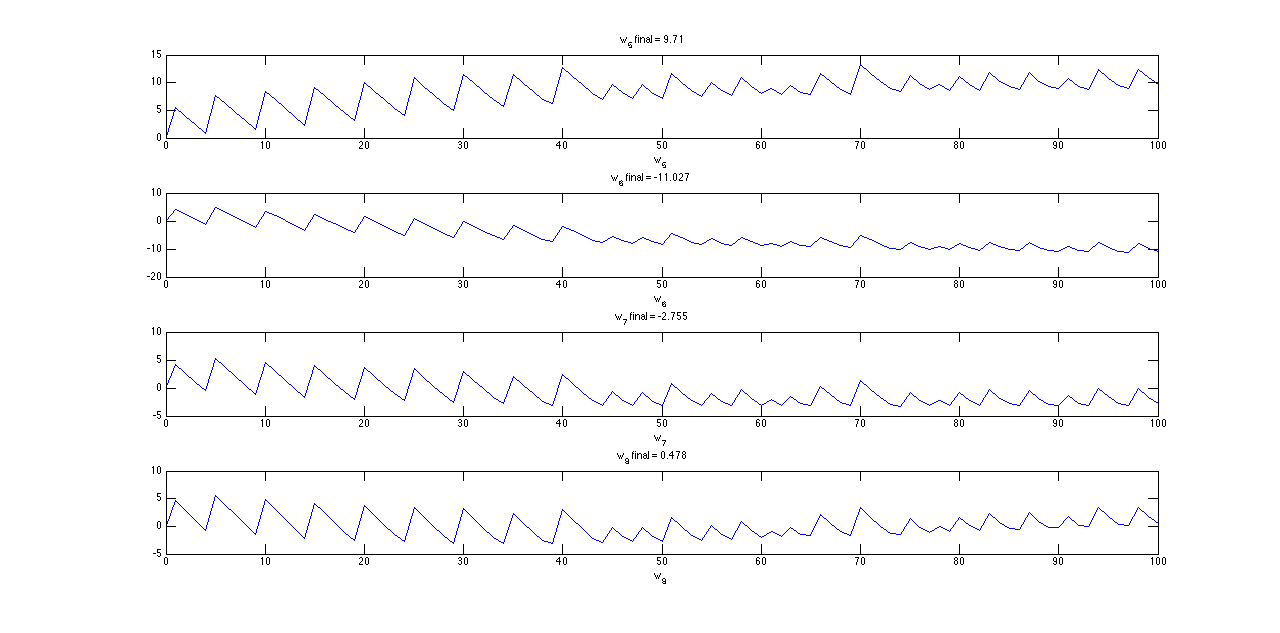
\includegraphics[width=26.5cm,height=8cm]{../res/part2_parametrogram2_init0.png}

\vspace*{-2em}
\hspace*{-13em}
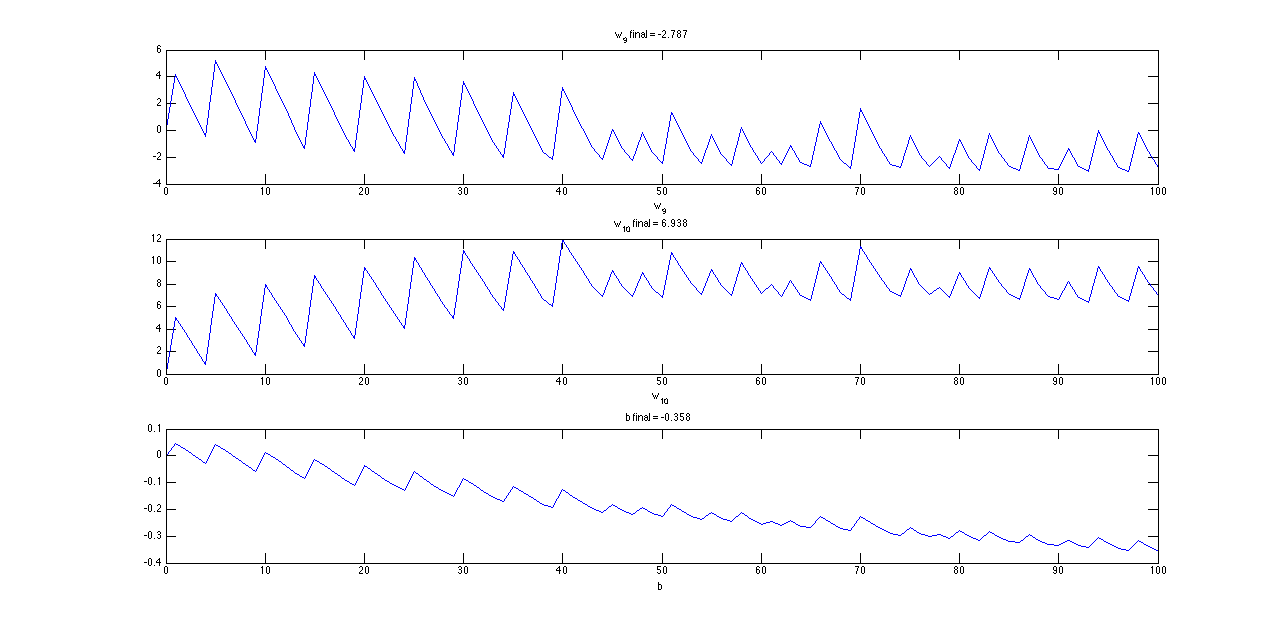
\includegraphics[width=26.5cm,height=6cm]{../res/part2_parametrogram3_init0.png}

\vspace*{-2em}
\begin{center}
[Fig.4: Parametrogram in part II]
\end{center}

\section*{Discussion}
\vspace{-20pt}
\noindent\makebox[\linewidth]{\rule{\textwidth}{0.4pt}}

\begin{enumerate}
	\item In the first part, does the final weight vector approximate the weights used for data generation (up to a scaling factor)?
	\begin{flushleft}
		In Fig.1, the final weight vector is $\begin{pmatrix}4.8209 \\ -3.621\\-8.4898 \\ 9.6843\end{pmatrix}$, which is roughly 
		paralleled to $\begin{pmatrix}0.4 \\ -0.3 \\ -0.7 \\ 0.8\end{pmatrix}$.
	\end{flushleft}
	\item Does the perceptron successfully (that is, with 100\% accuracy) separate the data into two classes?
	\begin{flushleft}
		Actually, it can successfully tell positive instances from negative ones. However, it usually requires a huge number of iterations 
		(more than 10,000 iterations) to improve little performance. Therefore, it is generally unable to completely separate the data into two 
		classes. (In general, the empirical error can be decreased to $1\%$ with only 
		hundreds of iterations)
	\end{flushleft}
	\item If not, does it help to repeatedly feed the whole set of data to your algorithm? (such as done in the for loop line 25)
	\begin{flushleft}
		According to perceptron convergence theorem, performance can achieve $100\%$ if two classes are linearly separable after large number of 
		iterations. Therefore, repeatedly feeding the whole set of data equivalently increase iterations, performance can be improved.
	\end{flushleft}
	\item In the starter code $\mathsf{Hw1\_starter.m}$, line16-17, the data are randomly sorted. What is the purpose of this, or does it matter?
	\begin{flushleft}
		In practice, randomly sorted data requires a smaller iterations to make the perceptron parameters converged, but it doesn't matter if we 
		iterate the learning algorithm with a large enough iterations. In short, randomly sorted data can generally accelerate convergence rate.
	\end{flushleft}
	\item In the second part, does the gender information help predicting whether a student passed or failed?
	\begin{flushleft}
		The weight of gender is $w_1$, and it is relatively small (-0.31) compared to other weights. Therefore, gender information is relatively irrelevant 
		to whether a student passed or failed in a course.
	\end{flushleft}
	\item Anything else worth mentioning.
	\begin{itemize}
		\item It also works if we update weights after feeding whole data rather than updating weights every time feeding a instance.
		\item The reason why the parametrogram of the second part doesn't converge is mainly that the size of data is too small to build 
			a learning system.
		\item If we apply a large data set of whether a student passed or failed, we can even predict grading rules and passed grade.
		\item More detailed implementation is available on \href{https://github.com/HW-Lee/2015-NN-Homeworks}
		{https://github.com/HW-Lee/2015-NN-Homeworks}.
	\end{itemize}
\end{enumerate}

\end{CJK}
\end{document}